%%%%%%%%%%%%%%%%%%%%%%%%%%%%%%%%%%%%%%%%%
% University/School Laboratory Report
% LaTeX Template
% Version 3.0 (4/2/13)
%
% This template has been downloaded from:
% http://www.LaTeXTemplates.com
%
% Original author:
% Linux and Unix Users Group at Virginia Tech Wiki 
% (https://vtluug.org/wiki/Example_LaTeX_chem_lab_report)
%
% License:
% CC BY-NC-SA 3.0 (http://creativecommons.org/licenses/by-nc-sa/3.0/)
%
%%%%%%%%%%%%%%%%%%%%%%%%%%%%%%%%%%%%%%%%%

%----------------------------------------------------------------------------------------
%	PACKAGES AND DOCUMENT CONFIGURATIONS
%----------------------------------------------------------------------------------------

\documentclass{article}

\usepackage[version=3]{mhchem} % Package for chemical equation typesetting
\usepackage{siunitx} % Provides the \SI{}{} command for typesetting SI units

\usepackage{graphicx}
\usepackage{caption}
\usepackage{subcaption}

\usepackage{float}

\usepackage[T1]{fontenc} % allow small bold caps

\usepackage{listings}
\usepackage{color}

\definecolor{dkgreen}{rgb}{0,0.6,0}
\definecolor{gray}{rgb}{0.5,0.5,0.5}
\definecolor{mauve}{rgb}{0.58,0,0.82}

\lstset{frame=tb,
  language=Python,
  aboveskip=2mm,
  belowskip=2mm,
  showstringspaces=false,
  columns=flexible,
  basicstyle={\small\ttfamily},
  numbers=none,
  numberstyle=\tiny\color{gray},
  keywordstyle=\color{blue},
  commentstyle=\color{dkgreen},
  stringstyle=\color{mauve},
  breaklines=true,
  breakatwhitespace=true
  tabsize=2
}

\setlength\parindent{0pt} % Removes all indentation from paragraphs

\renewcommand{\labelenumi}{\alph{enumi}.} % Make numbering in the enumerate environment by letter rather than number (e.g. section 6)

\usepackage[margin=1in]{geometry}

\usepackage{amssymb}

%\usepackage{times} % Uncomment to use the Times New Roman font

%----------------------------------------------------------------------------------------
%	Title
%----------------------------------------------------------------------------------------

\begin{document}
\pagenumbering{gobble}

\title{6.036: Machine Learning}
\author{
  Ryan Lacey <rlacey@mit.edu>\\
}
        
\maketitle
        

\begin{enumerate}
\item[1.] Using an offset did not reduce training error of the averager classifier. In fact it increased the number of misclassifications.

\bigskip

\item[3.] One set of data has wide margins and while the other set has a small margin between two oppositely labeled points. The first data set is easily separable and each classifier is able to find a linear boundary for the data. This could lead to the false assumption that they perform approximately the same, but the second data set puts this idea to rest. The averager classifier completely fails to separate the data. The perceptron result finds a decision boundary, but the boundary nearly lies on top of one of the data points. The passive-aggressive algorithm not only finds a separator, but finds one with near equidistant margins from the closely located points with opposite labels. \\
\bigskip
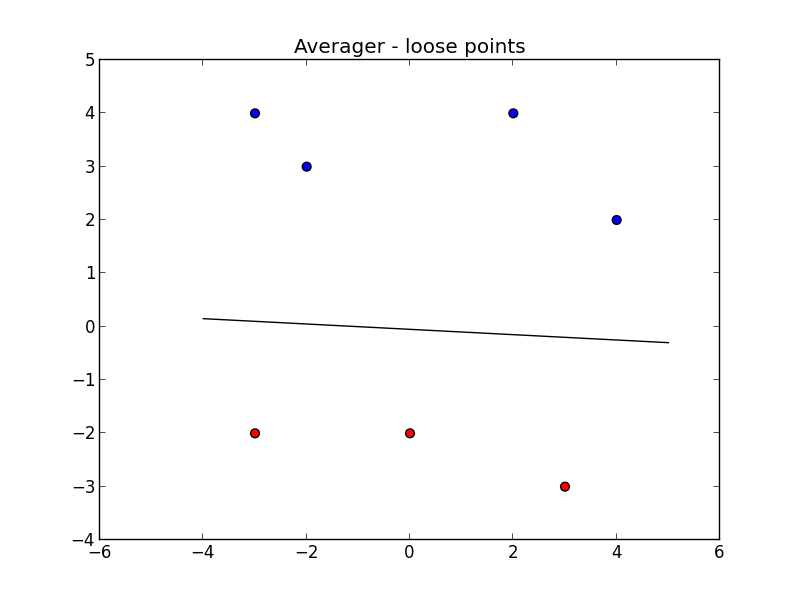
\includegraphics[width=\linewidth/3]{../Plots/AvgLoo} 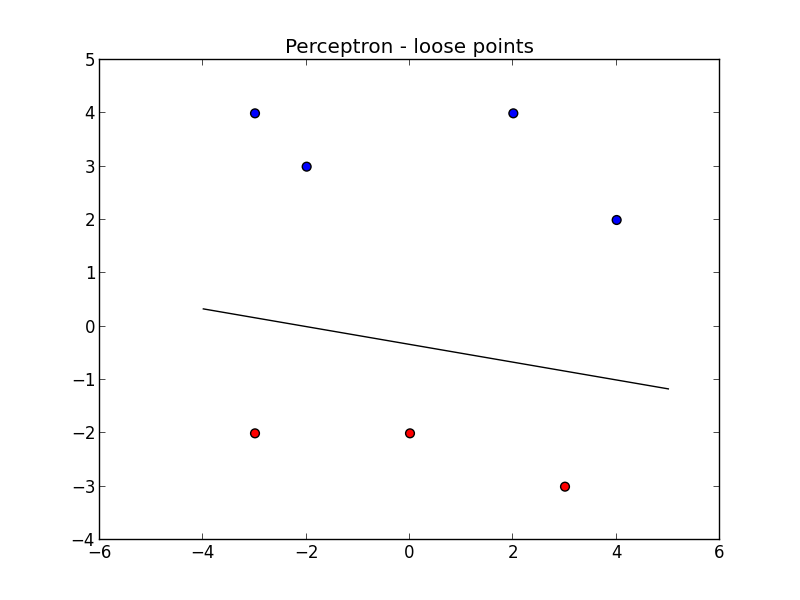
\includegraphics[width=\linewidth/3]{../Plots/PerLoo} 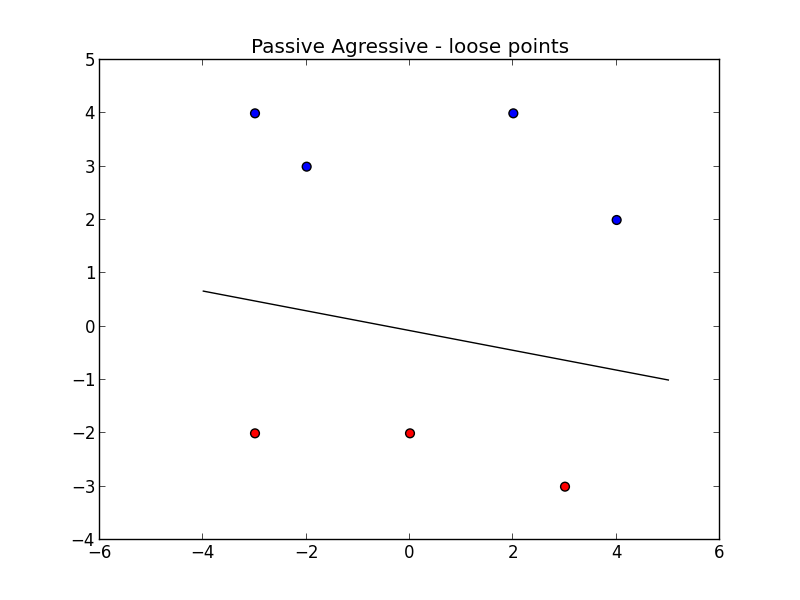
\includegraphics[width=\linewidth/3]{../Plots/PaLoo} \\
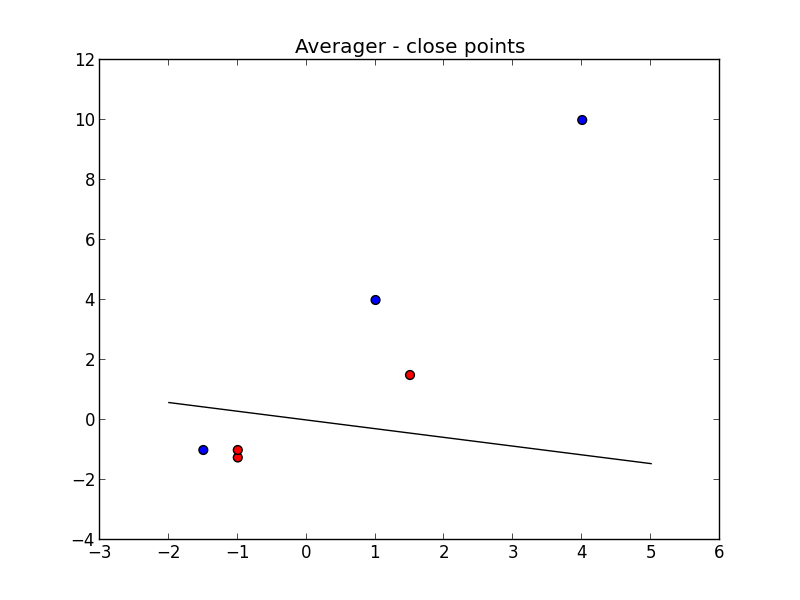
\includegraphics[width=\linewidth/3]{../Plots/AvgClo} 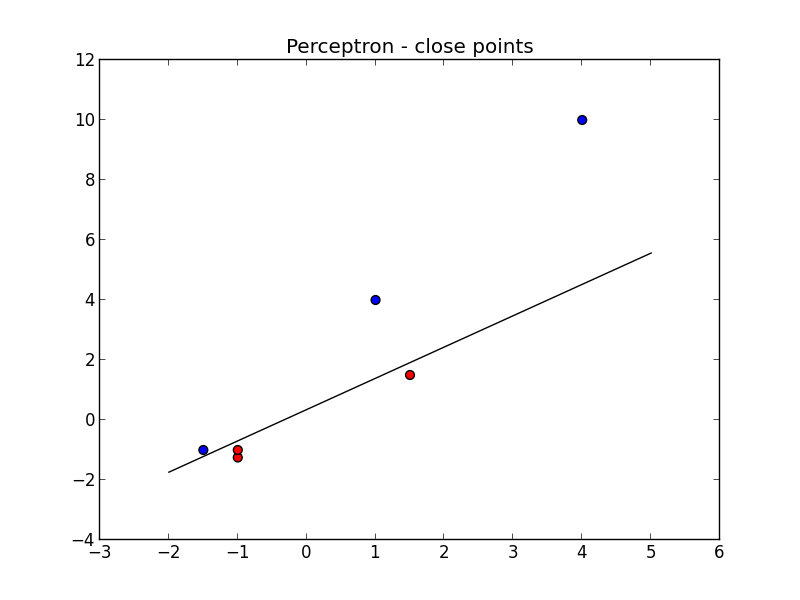
\includegraphics[width=\linewidth/3]{../Plots/PerClo} 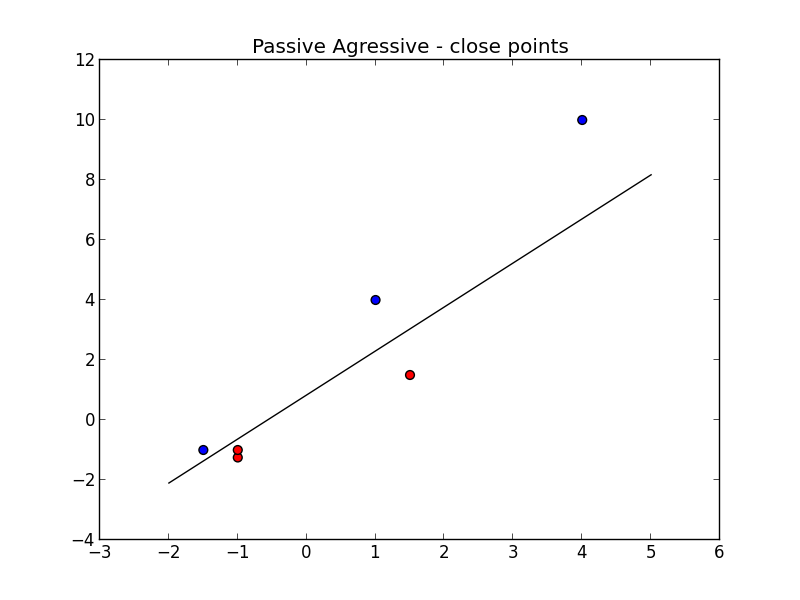
\includegraphics[width=\linewidth/3]{../Plots/PaClo} \\

\bigskip

\item[4.] I ran cross validation with $K=40$ for both the perceptron and passive-aggressive algorithms. On the standard feature set the average number of misclassifications were: \texttt{Perceptron: 83.67\%} and \texttt{Passive-Agressive: 83.17\%}. Using my modified feature set, described in \texttt{(6)}, the average misclassifications were: \texttt{Perceptron: 80.67\%} and \texttt{Passive-Agressive: 84.83\%}. The algorithms performed comparably on the given data and I would not say that one was conclusively superior to the other. Factors that influenced these results included: the value chosen for $K$ and the resulting training/test data subsets; the value chosen for $T$, which allows the passive-aggressive algorithm more iterations to try to reach an optimal solution; and the selection of feature to classify upon. 

\newpage

\item[5.] Machine learning classification lets a computer make educated guesses about the type of a thing. For this project the thing we were studying was "tweets" and the types were "positive" and "negative", describing the disposition of the tweet. To make these guesses the computer reads a lot of tweets which it knows are positive or negative and learns what words in them make the tweets that way. For example, if the word "terrific" was almost exclusively in tweets that were positive, then if the computer saw the word "terrific" in a new tweet it would make an educated guess that the new tweet is a positive one. Thus the computer has, in a sense, learned the disposition of various words.

\bigskip

\item[6.] My function \texttt{extract\_feature\_vectors\_with\_keywords} modifies the original feature set by weighting features. I provide a text file 'adjectives.txt' that contains a list of adjectives, adverbs, and other words with semantic meaning. When building the feature matrix I maintain the behavior of the original feature matrix building function \texttt{extract\_feature\_vectors} by giving value 0 to words not contained in the tweet. For words that are in the tweet, however, if it is one of the adjective words then it will receive a value of 2 and otherwise receive a value of 1 as before. The implementation of this function is shown below.

\bigskip 

\begin{lstlisting}   
def extract_feature_vectors_with_keywords(file, dict, keys):
    """
      Returns a bag-of-words representation of a text file, given a dictionary.
      The returned matrix is of shape (m, n), where the text file has m non-blank
      lines, and the dictionary has n entries.
    """
    f = open(file, 'r')
    num_lines = 0
    for line in f:
        if(line.strip()):
            num_lines = num_lines + 1
    f.close()
    feature_matrix = np.zeros([num_lines, len(dict)])
    f = open(file, 'r')
    pos = 0
    for line in f:
        if(line.strip()):
            flist = extract_words(line)
            for word in flist:
                if(word in dict):
                    if word in keys:
                        feature_matrix[pos, dict.index(word)] = 2
                    else:
                        feature_matrix[pos, dict.index(word)] = 1
            pos = pos + 1
    f.close()
    return feature_matrix
\end{lstlisting}

\bigskip

 The goal was to give words that are likely to express disposition (words such as good, terrible, best, etc.) greater influence in classification. I ran cross validation on the original feature matrix with a correct average classification of 83.2\% for the passive-aggressive algorithm and on my modified feature matrix with a correct average classification of 84.9\% for the same algorithm. Thus performance improved using my new feature set.
 
\end{enumerate}

\end{document}